\subsection{The Trapdoor Random Oracle}

The above protocol in which the $ctr$ of each block remains secret can be
abstracted by the concept of a \emph{trapdoor random oracle} in which the party
that mines a new block makes the first query to the random oracle using a
\emph{secret witness} $sw$ which is associated with a unique
\emph{public witness} $pw$. The random oracle returns a response $y$ as usual,
but also associates a secret $\xi$ with this response, following a distribution
$\Xi$ which is predetermined. The secret $\xi$ is only recoverable and
verifiable using the secret witness $sw$. In our protocol, an honest miner
reveals $sw$ at a later time in order to prove to other parties whether their
previously mined block is a $Q$-block. The $Q$-blockness of a block is then
determined by any predicate applied on $\xi$. The adversary can, of course, keep
the secret witness $sw$ withheld.

\import{./}{chapters/superlight/algorithms/trapdoor-ro.tex}

\begin{figure*}
\fbox{
	\begin{minipage}{0.9 \textwidth}
  The \emph{trapdoor} random oracle functionality $\textsc{RO}_\Xi$ is
  parameterized by the security parameters $\kappa, \lambda$ and a distribution
  ensemble $(\Xi)_\kappa$. Upon initialization, it sets $T_p$ and $T_f$ to
  $\emptyset$. It supplies the following methods:

	\begin{itemize}
			\item $\textsc{query-f}(sw)$:
            If $(sw, pw) \in T_f$ for some value $pw$, return $pw$.
            Otherwise choose a
            $pw \gets \{0, 1\}^\lambda$ and set
            $T_f = T_f \cup \{(sw, pw)\}$, then return $pw$.
      \item $\textsc{query-p}(x)$:
            If $(x, y, \xi) \in T_p$ for some
            values $y, \xi$, return $y$.
            Otherwise choose
            $y \gets \{0, 1\}^\kappa$ and
						$\xi \gets \Xi_\kappa$ and set
            $T_p = T_p \cup \{(x, y, \xi)\}$, then
            return $y$.
      \item $\textsc{query-s}(x, sw)$:
					  Parse $x = x'||pw$ for some $x', pw$.
						If the parsing fails, return $\bot$.
						Otherwise, if $\textsc{query-f}(pw) \neq sw$, then the
						trapdoor is incorrect, so return $\bot$.
						Otherwise, if $(x, y, \xi) \in T_s$ for some values
            $y, \xi$, return $\xi$.
            Otherwise, choose
						$y \gets \{0, 1\}^\kappa$ and
            $\xi \gets \Xi_\kappa$ and set
            $T_s = T_s \cup \{(x, y, \xi)\}$, then return $\xi$.
	\end{itemize}

	\end{minipage}
}
\caption{
The \emph{trapdoor} random oracle functionality $\textsc{RO}_\Xi$.
\label{fig:trapdoor-ro}
}
\end{figure*}

\begin{figure}[h]
\begin{center}
  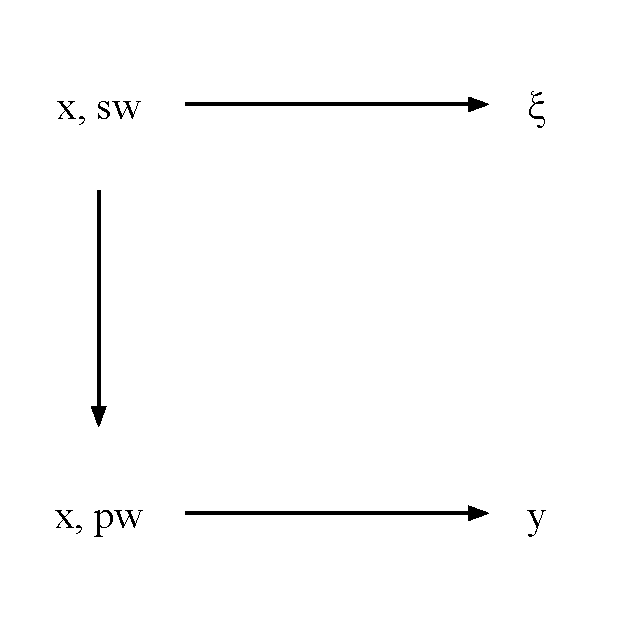
\includegraphics[width=0.30\textwidth]{chapters/superlight/figures/rox-commutative-diagram.pdf}
  \caption{The $\textsc{RO}_\Xi$ functionality and the directions of its available queries.}
  \label{fig:rox-commutativity-diagram}
  \end{center}
\end{figure}

The Trapdoor Random Oracle is illustrated in Figure~\ref{fig:trapdoor-ro} and
works as follows. A query is made to the Random Oracle by invoking the
$\textsc{query-p}$ or $\textsc{query-s}$ methods, passing an $x$
(the query string) as well as a public
witness $pw$ (for $\textsc{query-p}$) or a secret witness $sw$ (for $\textsc{query-s}$). The
public query returns $y$, while the private query returns $\xi$. If the
invocation is not new, the method returns the cached value. Otherwise, the
extended Random Oracle functionality generates a $y$ uniformly at random as
usual for the public query. In addition, it generates a value $\xi$ by sampling
from the distribution $\Xi$ for the private query. It also provides a
functionality $\textsc{query-f}$ which allows retrieving $pw$ given $sw$. The
query directions offered by the functionality are depicted in
Figure~\ref{fig:rox-commutativity-diagram}.

Next we show how the trapdoor random oracle can be implemented
for a distribution ensemble equal to $\{0,1\}^\kappa$.
Then we have the following theorem:

\begin{theorem}
 Algorithm~\ref{alg.trapdoor-ro-imp} implements the functionality
 $\textsc{RO}_\Xi$ in Figure
  \ref{fig:rox-commutativity-diagram} assuming random oracles $G,H$.
\end{theorem}

\import{./}{chapters/superlight/algorithms/trapdoor-ro-imp.tex}

Given the above functionality, block generation can be performed as usual, but
invoking the Trapdoor Random Oracle to perform blinded mining. In this case, the
input to the Trapdoor Random Oracle includes all of the usual data
($ctr || x || s$) as well as a secret witness $sw$ which is revealed at a later
time.

\noindent
\textbf{Remark.}
In practice, our scheme can be implemented using the following technique to
avoid commitments. Query $H(H(ctr) || x || s) \leq T$ to check if the query gives
a valid block. If so, then reveal $H(ctr) || x || s$. Anyone on the network can
check the block's validity. Whether the block is a Q-block can be determined by
checking whether, for some $\mu \in \mathbb{N}$ the following inequality holds:

\[
  H(ctr || H(H(ctr) || x || s)) \leq 2^{-\mu}
\]

This can only be checked once $ctr$ is revealed (provided $ctr$ contains
sufficient entropy), which corresponds to the Trapdoor Random Oracle secret.
The particular order of evaluation for $H$ ensures that the query for block
validity $H(H(ctr) || x || s)$ has to be submitted by the adversary before they
are able to learn the Q-status of the block through the query
$H(ctr || H(H(ctr) || x || s))$.
